\documentclass[border=10pt]{standalone}
\usepackage[svgnames]{xcolor}
\usepackage{amsmath}
\usepackage{pgfplots}
\pgfplotsset{compat=newest}
\usepackage[sfdefault]{FiraSans}
\usepackage{FiraMono}
\renewcommand*\familydefault{\sfdefault}
\begin{document}
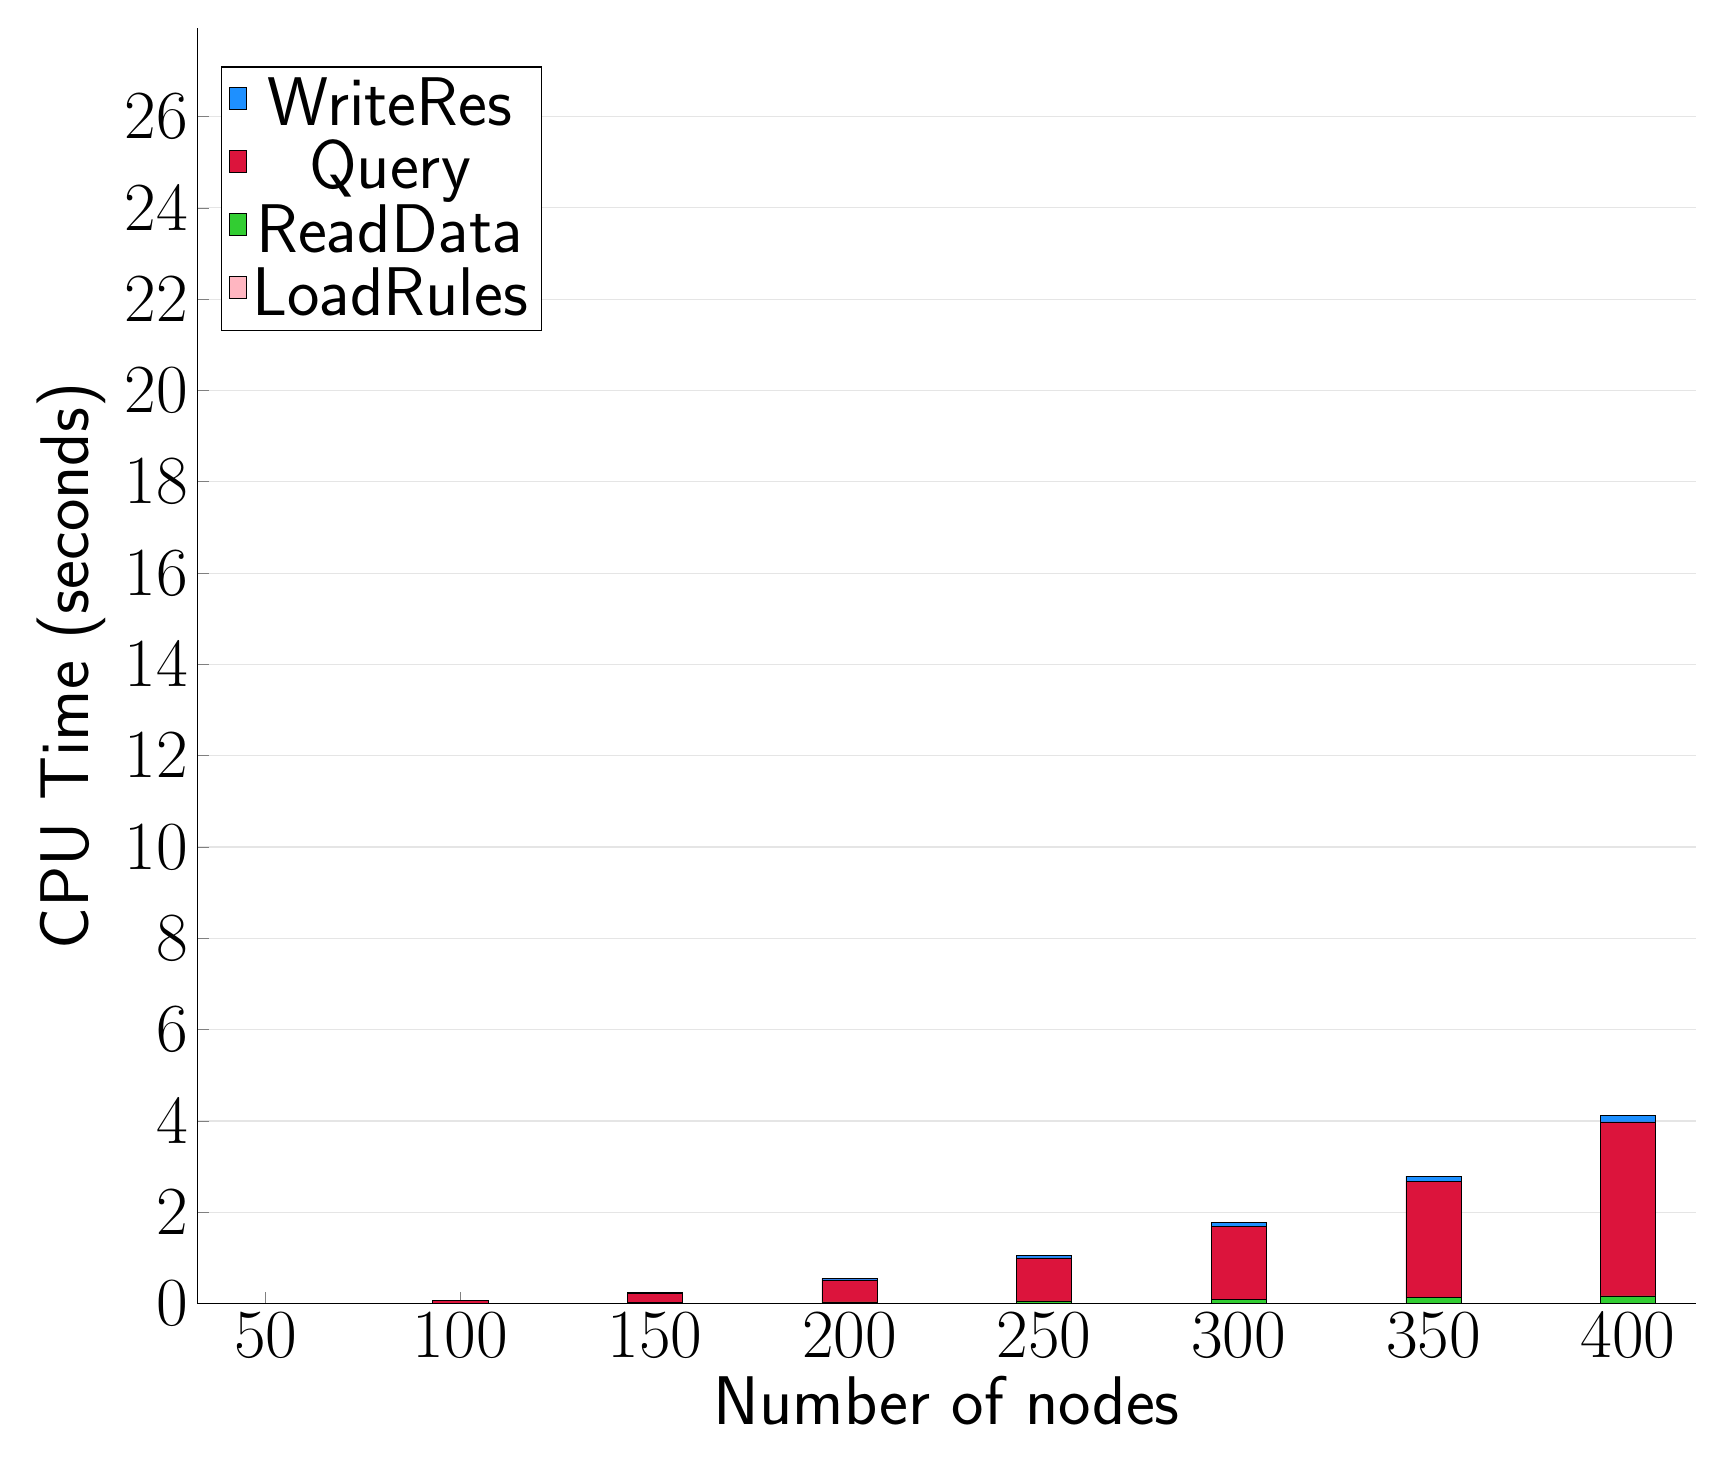
\begin{tikzpicture}
\begin{axis}[
   ybar stacked,
   width=1.7\textwidth,
   bar width=0.7cm,
   ymajorgrids, tick align=inside,
   major grid style={draw=gray!20},
   xtick=data,
   ymin=0, ymax=27.933910000000004,
   axis x line*=bottom,
   axis y line*=left,
   enlarge x limits=0.05,
   legend style={
       at={(0.23, 0.97)},
       anchor=north east,
       legend columns=1,
       font=\Huge,
   },
   ylabel={CPU Time (seconds)},
   xlabel={Number of nodes},
   label style={font=\Huge},
   tick label style={font=\Huge},
]
\addlegendimage{fill=DodgerBlue, draw=black, line width=0.2pt}
\addlegendentry{WriteRes}
\addlegendimage{fill=Crimson, draw=black, line width=0.2pt}
\addlegendentry{Query}
\addlegendimage{fill=LimeGreen, draw=black, line width=0.2pt}
\addlegendentry{ReadData}
\addlegendimage{fill=LightPink, draw=black, line width=0.2pt}
\addlegendentry{LoadRules}
\addplot +[fill=LightPink, draw=black, line width=0.2pt] coordinates {
(50, 0.0005436999999999999)
(100, 0.0006297)
(150, 0.0006088999999999999)
(200, 0.0006082000000000001)
(250, 0.0006123999999999998)
(300, 0.0006215000000000003)
(350, 0.0006266999999999999)
(400, 0.0006372000000000003)
};
\addplot +[fill=LimeGreen, draw=black, line width=0.2pt] coordinates {
(50, 0.0023761999999999998)
(100, 0.0088507)
(150, 0.0206731)
(200, 0.0383251)
(250, 0.061571799999999996)
(300, 0.0910103)
(350, 0.12799129999999997)
(400, 0.1706672)
};
\addplot +[fill=Crimson, draw=black, line width=0.2pt] coordinates {
(50, 0.0077931)
(100, 0.059859300000000004)
(150, 0.20364539999999995)
(200, 0.48165009999999997)
(250, 0.9390012999999999)
(300, 1.6043246)
(350, 2.5467262000000006)
(400, 3.8088134000000005)
};
\addplot +[fill=DodgerBlue, draw=black, line width=0.2pt] coordinates {
(50, 0.0022654999999999997)
(100, 0.0090485)
(150, 0.022953)
(200, 0.03450349999999998)
(250, 0.0557735)
(300, 0.07931240000000002)
(350, 0.1196857)
(400, 0.1429398)
};
\end{axis}
\end{tikzpicture}

\end{document}
